\documentclass[12pt,a4paper]{report}
\usepackage[utf8]{inputenc}
\usepackage[T1]{fontenc}
\usepackage{mathptmx}
\usepackage[top=2.5cm,bottom=2.5cm,left=3cm,right=2.5cm,headheight=14pt,headsep=18pt,footskip=30pt]{geometry}
\usepackage{setspace}
\usepackage{fancyhdr}
\usepackage{graphicx}
\usepackage{tabularx}
\usepackage[table]{xcolor}
\usepackage[hidelinks]{hyperref}
\onehalfspacing

\pagestyle{fancy}
\fancyhf{}
\fancyhead[L]{Mini-API Assurance --- Vermeg}
\fancyhead[R]{Taher Yahia}
\fancyfoot[C]{\thepage}
\renewcommand{\headrulewidth}{0pt}

\setlength{\parindent}{0pt}
\setlength{\parskip}{6pt}

\title{\textbf{Conception et réalisation d'une mini-API REST de gestion d'assurance}}
\author{Taher Yahia}
\begin{document}

\begin{titlepage}
\begin{center}

\includegraphics[height=2.4cm]{logos/logo-universite-gabes.png}\hfill

\includegraphics[height=2.4cm]{logos/logo-isimg.jpg}\hfill

\includegraphics[height=2.4cm]{logos/logo-vermeg.png}\hfill\par\vspace{1cm}
\textbf{République Tunisienne}\\
\textbf{Ministère de l'Enseignement Supérieur et de la Recherche Scientifique}\\
\textbf{Université de Gabès}\\
\textbf{Institut Supérieur d'Informatique et de Multimédia de Gabès}\\[2cm]
\textbf{Rapport de stage d'initiation}\\[0.4cm]
\emph{Licence Fondamentale en Informatique --- Génie Logiciel (FIGL), première année}\\[1.5cm]
{\LARGE \textbf{Conception et réalisation d'une mini-API REST de gestion d'assurance}\par}\vspace{1.5cm}
\textbf{Réalisé par :} Taher Yahia\\[0.3cm]
\textbf{Organisme d'accueil :} Vermeg\\
\textbf{Encadrante entreprise :} Mme Faten Kardous, \emph{Lead Developer}, Insurance Market Operations\\
\textbf{Période :} du 1\textsuperscript{er} au 31 juillet 2026\\
\textbf{Année universitaire :} 2025 / 2026
\end{center}
\end{titlepage}


\newpage
\chapter*{Remerciements}
\addcontentsline{toc}{chapter}{Remerciements}
Je remercie Mme Faten Kardous, \textit{Lead Developer} au sein du département Insurance Market Operations de Vermeg, pour son encadrement, sa disponibilité et la clarté des objectifs qu'elle m'a fixés.
Je remercie les collaborateurs de Vermeg que j'ai côtoyés pour leur accueil et leurs conseils, ainsi que le corps enseignant de l'Institut Supérieur d'Informatique et de Multimédia de Gabès, dont la formation de première année a constitué la base directe des travaux présentés ici.
Je remercie enfin les membres du jury pour l'attention portée à ce document.
\newpage
\chapter*{Table des matières}
\tableofcontents
\listoffigures
\listoftables
\addcontentsline{toc}{chapter}{Table des matières}
\newpage
\chapter*{Introduction}
\addcontentsline{toc}{chapter}{Introduction}
Le cursus de licence en informatique de l'Institut Supérieur d'Informatique et de Multimédia de Gabès prévoit un stage d'initiation d'une durée minimale de quatre semaines continues. Ce stage vise à découvrir l'organisation réelle d'une entreprise du secteur, à mettre en pratique les acquis de première année et à produire un document professionnel rendant compte du travail effectué.
J'ai effectué ce stage du 1er au 31 juillet 2026 chez Vermeg, éditeur de solutions logicielles pour les services financiers et l'assurance, sous l'encadrement de Mme Faten Kardous, \textit{Lead Developer} au département Insurance Market Operations. Les formalités administratives associées — convention, fiche de suivi, attestation — ont été traitées séparément et ne font pas l'objet de ce rapport.
Le sujet confié porte sur la réalisation d'une \textbf{mini-API REST de gestion d'assurance}~: construire, à partir de zéro, un service web gérant les objets élémentaires d'un système assurantiel — clients, contrats et sinistres — en respectant les pratiques en vigueur dans l'entreprise. La problématique peut se formuler ainsi~: \textit{comment exposer, de manière sûre, cohérente et documentée, les opérations de gestion d'un portefeuille d'assurance élémentaire, tout en garantissant le respect des règles qui lient un sinistre à son contrat et un contrat à son client~?}
Six objectifs opérationnels ont été fixés~: modéliser le domaine sous forme d'entités persistantes~; exposer une API REST couvrant clients, contrats et sinistres~; faire respecter les règles métier par le serveur plutôt que par le client~; sécuriser les accès par jeton~; documenter l'interface de manière interactive~; rendre l'environnement d'exécution reproductible.
Le rapport suit six chapitres~: présentation de l'entreprise et du cadre du stage, analyse du besoin, conception, réalisation technique, vérification et regard critique, puis bilan au regard de la formation.
\newpage
\chapter*{Chapitre 1 — Présentation de l'entreprise et cadre du stage}
\addcontentsline{toc}{chapter}{Chapitre 1 — Présentation de l'entreprise et cadre du stage}
\section*{1.1. Présentation de Vermeg}
\addcontentsline{toc}{section}{1.1. Présentation de Vermeg}
Vermeg est un éditeur de solutions logicielles spécialisé dans les services financiers, dont l'offre couvre la banque, les marchés de capitaux, la gestion d'actifs et l'assurance [1], [2]. Fondée en 1993 en Tunisie sous le nom de BFI, dont elle a été détachée en 2002, l'entreprise a aujourd'hui son siège à Amsterdam et dispose d'implantations sur plusieurs continents, dont la Tunisie [2]. Son activité consiste à fournir aux institutions financières des progiciels métier et des développements sur mesure~: gestion de portefeuilles, reporting réglementaire, gestion du collatéral et gestion de polices d'assurance [1], [2].
Le département qui m'a accueilli, \textbf{Insurance Market Operations}, intervient sur le segment assurance. Cette spécialisation explique le sujet confié~: travailler sur les objets métier fondamentaux de l'assurance permet de se familiariser avec le vocabulaire et la logique du domaine dans lequel l'équipe évolue quotidiennement.
\textit{Les données relatives à l'organigramme, à l'effectif du site et aux résultats financiers n'ont pas été communiquées dans un cadre exploitable et ne sont donc pas reproduites ici.}
\section*{1.2. Cadre et organisation du stage}
\addcontentsline{toc}{section}{1.2. Cadre et organisation du stage}
Le stage s'est déroulé sur quatre semaines pleines et continues, du 1er au 31 juillet 2026, conformément à la durée minimale exigée par l'institut. L'organisation a reposé sur un rythme itératif~: un objectif fonctionnel par période de quelques jours, une réalisation autonome, puis un point de validation avec l'encadrante. Le découpage suivi a été le suivant.
\textbf{Semaine 1}~: prise de connaissance du domaine et de l'écosystème Spring Boot, initialisation du projet, modélisation des entités et persistance. \textbf{Semaine 2}~: couches service et contrôleur pour les clients et les contrats, objets de transfert et validation des entrées. \textbf{Semaine 3}~: sinistres et règles associées, sécurisation par jeton, documentation OpenAPI, gestion des erreurs. \textbf{Semaine 4}~: conteneurisation, premier test unitaire, travail personnel sur un client web Angular, rédaction du rapport.
\section*{1.3. Sujet et objectifs}
\addcontentsline{toc}{section}{1.3. Sujet et objectifs}
Le sujet consiste à développer une interface de programmation REST autonome, sans dépendance à un système existant de l'entreprise, gérant trois ressources métier reliées~: clients, contrats et sinistres. L'accent porte sur le \textbf{backend}~: le cahier des charges visait un service serveur correct, structuré et sécurisé, et non une interface graphique. Cette orientation est cohérente avec l'objectif pédagogique — consolider la programmation orientée objet, la persistance relationnelle et la conception d'API avant d'aborder les couches de présentation.
\section*{1.4. Méthodologie de travail}
\addcontentsline{toc}{section}{1.4. Méthodologie de travail}
J'ai utilisé Git avec un dépôt distant sur GitHub, en conservant la branche principale dans un état fonctionnel et en isolant les développements exploratoires sur des branches dédiées~: le client web Angular, mené hors du périmètre initial, a été développé sur une branche séparée afin de ne pas déstabiliser le backend validé. Les messages de commit suivent la convention \textit{Conventional Commits} [3], qui préfixe le message par le type de changement (\texttt{feat}, \texttt{fix}, \texttt{test}, \texttt{docs}). Le dernier commit du dépôt, \texttt{feat(frontend): page gestion employés (ADMIN) + roleGuard + UI conditionnelle}, en illustre l'usage. Cette convention rend l'historique lisible et permet de retrouver rapidement le contexte d'une modification~; c'est une pratique professionnelle que je n'appliquais pas avant ce stage.
Outils employés~: IntelliJ IDEA pour Java, Visual Studio Code pour Angular, \texttt{psql} et pgAdmin pour l'inspection de la base, Swagger UI et Postman pour l'appel des points d'accès, Docker Desktop pour l'exécution conteneurisée.
\textit{Le cadre étant posé, le chapitre suivant précise le besoin et le délimite.}
\newpage
\chapter*{Chapitre 2 — Contexte et analyse du besoin}
\addcontentsline{toc}{chapter}{Chapitre 2 — Contexte et analyse du besoin}
\section*{2.1. Contexte métier}
\addcontentsline{toc}{section}{2.1. Contexte métier}
Un système d'assurance repose sur trois objets fondamentaux, reliés par des dépendances d'existence. Le \textbf{client} est la personne physique assurée, identifiée de manière unique par sa carte d'identité nationale. Le \textbf{contrat}, ou police, est la garantie souscrite par un client~: il porte un type, une période de validité, un montant couvert et une prime. Le \textbf{sinistre} est l'événement dommageable déclaré au titre d'un contrat~; il porte une date de survenance, une date de déclaration, un montant estimé et un statut d'instruction.
La cohérence de cet ensemble repose sur des invariants simples mais impératifs~: un sinistre ne peut exister sans contrat, un contrat sans client, et un sinistre ne peut être déclaré que sur un contrat en cours de validité au moment des faits. Le rôle du serveur est de garantir ces invariants indépendamment du client appelant.
\section*{2.2. Besoins fonctionnels}
\addcontentsline{toc}{section}{2.2. Besoins fonctionnels}
\begin{center}\textit{Tableau 1 — Besoins fonctionnels retenus et état de réalisation}\end{center}
{\small
\begin{tabularx}{\linewidth}{|X|X|X|}
\hline
\textbf{Réf.} & \textbf{Besoin} & \textbf{État} \\ \hline
BF1 & Créer un compte utilisateur doté d'un rôle & Réalisé \\ \hline
BF2 & S'authentifier et obtenir un jeton d'accès & Réalisé \\ \hline
BF3 & Créer, consulter et modifier un client & Réalisé \\ \hline
BF4 & Archiver un client sans le supprimer physiquement & Réalisé \\ \hline
BF5 & Interdire l'archivage d'un client encore rattaché à un contrat & \textbf{Non réalisé} — voir 5.4 \\ \hline
BF6 & Créer un contrat pour un client existant & Réalisé \\ \hline
BF7 & Consulter la liste et le détail des contrats, y compris par client & Réalisé \\ \hline
BF8 & Mettre à jour un contrat (montants, échéance, statut) & Réalisé \\ \hline
BF9 & Déclarer un sinistre sur un contrat, avec justificatif & Réalisé \\ \hline
BF10 & Consulter les sinistres d'un contrat, tous les sinistres, ou un sinistre & Réalisé \\ \hline
BF11 & Consulter la liste des employés de l'application & Réalisé, réservé à l'administrateur \\ \hline
BF12 & Instruire un sinistre (transitions de statut, remboursement) & Non retenu — reporté \\ \hline
\end{tabularx}

}
Deux lignes appellent un commentaire. \textbf{BF5} a été identifié à l'analyse et préparé dans le code — une méthode de vérification \texttt{existsByClientId} existe dans la couche d'accès aux données — mais le contrôle n'a finalement pas été branché sur l'opération d'archivage~; cette lacune est documentée en section 5.4 plutôt que passée sous silence. \textbf{BF12} a été écarté du périmètre~: il suppose un modèle de workflow d'instruction dont la définition dépassait le temps disponible, et il figure dans les perspectives (section 6.3).
\section*{2.3. Besoins non fonctionnels}
\addcontentsline{toc}{section}{2.3. Besoins non fonctionnels}
\textbf{Sécurité}~: aucune ressource métier accessible sans authentification, aucun mot de passe stocké en clair. \textbf{Intégrité}~: les contraintes d'unicité et de non-nullité doivent être portées par le schéma relationnel et non seulement par le code. \textbf{Validation}~: toute donnée entrante doit être vérifiée avant traitement, avec un retour exploitable. \textbf{Documentation}~: l'interface doit être auto-documentée et testable sans outil externe. \textbf{Portabilité}~: l'application doit démarrer sur un poste tiers avec un minimum d'installation. \textbf{Absence d'état de session}~: le service doit rester sans état, afin de demeurer simple à répliquer.
\section*{2.4. Périmètre retenu et hors-périmètre}
\addcontentsline{toc}{section}{2.4. Périmètre retenu et hors-périmètre}
Le périmètre demandé se limite au \textbf{backend}~: l'API REST, sa persistance, sa sécurité et sa documentation. La conteneurisation y a été ajoutée en cours de stage pour répondre au besoin de portabilité.
Une \textbf{interface web Angular} a par ailleurs été développée. Il s'agit d'une \textbf{initiative personnelle}, entreprise en fin de stage, dans un objectif de montée en compétences~: découvrir un framework front-end et vérifier concrètement que l'API produite était consommable par un client réel, notamment sur les aspects de politique d'origine croisée et de transmission du jeton. Ce travail n'était pas une exigence de l'entreprise~; son état d'avancement réel est décrit sans complaisance en section 4.8.
Sont explicitement hors-périmètre~: la gestion des primes et échéanciers, le workflow d'instruction des sinistres, l'édition de documents contractuels, l'intégration à un système d'information existant, la pagination des listes et tout déploiement en production.
\textit{Le besoin étant délimité, le chapitre suivant présente les choix de conception.}
\newpage
\chapter*{Chapitre 3 — Conception}
\addcontentsline{toc}{chapter}{Chapitre 3 — Conception}
\section*{3.1. Architecture globale}
\addcontentsline{toc}{section}{3.1. Architecture globale}
L'application suit une architecture en couches, où chaque couche ne dialogue qu'avec sa voisine immédiate (figure 1). Une requête émise par un client HTTP traverse d'abord la chaîne de filtres de sécurité, atteint un contrôleur qui délègue le traitement à un service~; le service applique les règles métier et sollicite un \textit{repository}, lequel dialogue avec PostgreSQL par l'intermédiaire de JPA.
\begin{figure}[htbp]\centering
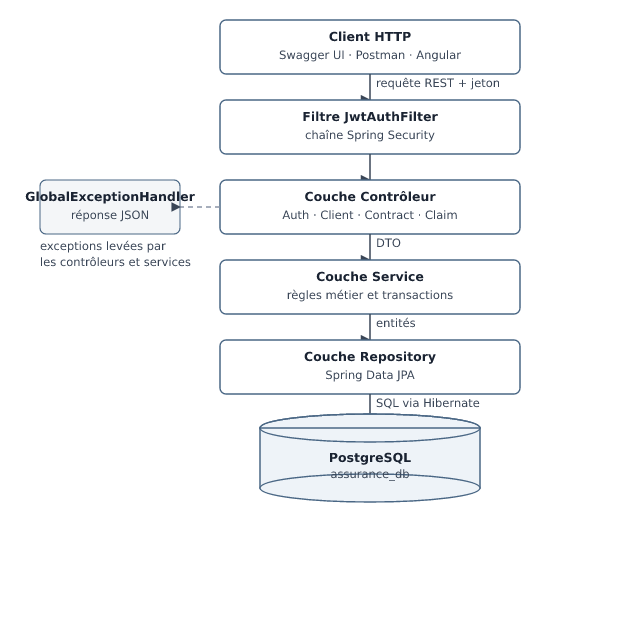
\includegraphics[width=0.95\linewidth]{figures/fig1.png}
\caption{Figure 1 — Architecture globale de la solution}
\end{figure}
Cette organisation applique le principe de séparation des responsabilités. Elle a produit deux bénéfices observables~: la logique métier reste testable indépendamment du transport HTTP, comme l'a montré l'écriture du test unitaire du service de sinistres (section 5.1)~; et une modification du contrat d'interface n'impacte pas le cœur métier tant que les objets de transfert sont conservés.
\section*{3.2. Modèle de domaine}
\addcontentsline{toc}{section}{3.2. Modèle de domaine}
Le modèle, représenté en figure 2, comporte quatre entités persistantes et quatre énumérations. Les relations sont de type « un-à-plusieurs »~: un client possède plusieurs contrats, un contrat porte plusieurs sinistres. L'entité \texttt{User}, dédiée à l'authentification et à l'autorisation, est indépendante du domaine assurance.
\begin{figure}[htbp]\centering
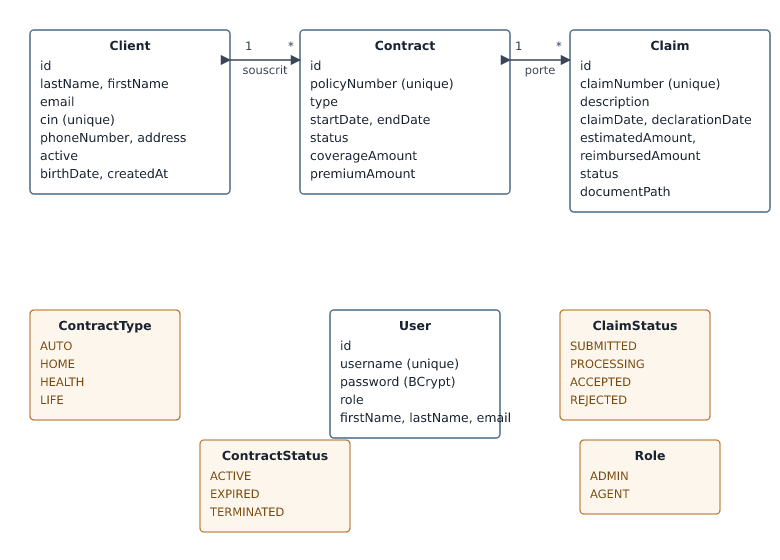
\includegraphics[width=0.95\linewidth]{figures/fig2.png}
\caption{Figure 2 — Modèle de domaine de l'application}
\end{figure}
Quatre décisions de modélisation méritent justification. Les \textbf{montants} sont typés \texttt{BigDecimal} et non \texttt{double}~: un flottant binaire ne représente pas exactement les valeurs décimales et introduit des erreurs d'arrondi inacceptables sur des montants financiers. Les \textbf{énumérations} sont persistées en chaînes de caractères et non par leur position ordinale~: le stockage ordinal rend la base illisible et surtout fragile, puisque l'insertion d'une valeur au milieu de l'énumération corromprait silencieusement les données existantes. Les \textbf{associations} sont chargées paresseusement afin d'éviter le chargement du graphe complet d'objets à chaque lecture~; ce choix impose en contrepartie que la conversion en objets de transfert ait lieu dans la transaction, contrainte à l'origine d'une difficulté détaillée en section 5.3. Enfin, le client comporte un \textbf{booléen d'archivage} plutôt qu'une suppression physique~: un client disparaît des listes sans que l'historique de ses contrats et de ses sinistres soit perdu, ce qui est la seule option acceptable pour des données à valeur juridique.
\section*{3.3. Architecture applicative en couches}
\addcontentsline{toc}{section}{3.3. Architecture applicative en couches}
Le code est organisé en paquetages fonctionnels sous \texttt{com.assurance.mini\_api\_assurance}~: \texttt{domain} (entités et énumérations), \texttt{dto} (objets de transfert), \texttt{mapper} (conversion entité vers DTO), \texttt{repository} (interfaces Spring Data), \texttt{service} (règles métier et transactions), \texttt{controller} (exposition HTTP), \texttt{security} (jetons et chargement des utilisateurs), \texttt{config} (sécurité, OpenAPI, données de démonstration) et \texttt{exception} (exceptions métier et gestionnaire global). L'ensemble représente 47 classes Java pour environ 1 800 lignes de code.
L'introduction de \textbf{DTO distincts des entités} est un choix structurant~: il évite d'exposer le modèle persistant — ce qui divulguerait des champs internes tels que le mot de passe haché — et permet des contrats d'entrée différenciés. \texttt{ClientCreateDto} exige ainsi le numéro de carte d'identité nationale, alors que \texttt{ClientUpdateDto} ne le contient pas, ce qui interdit techniquement la modification d'un identifiant national après création. De même, le chemin interne du justificatif téléversé n'apparaît dans aucune réponse.
\section*{3.4. Conception de la sécurité}
\addcontentsline{toc}{section}{3.4. Conception de la sécurité}
L'authentification repose sur le standard JSON Web Token défini par la RFC 7519 [4]. L'utilisateur s'authentifie une fois par identifiant et mot de passe, reçoit un jeton signé, puis le présente à chaque requête ultérieure dans l'en-tête \texttt{Authorization}. Le serveur ne conserve aucune session~: il vérifie la signature et l'expiration à chaque appel. La figure 3 détaille les deux temps de cet échange.
\begin{figure}[htbp]\centering
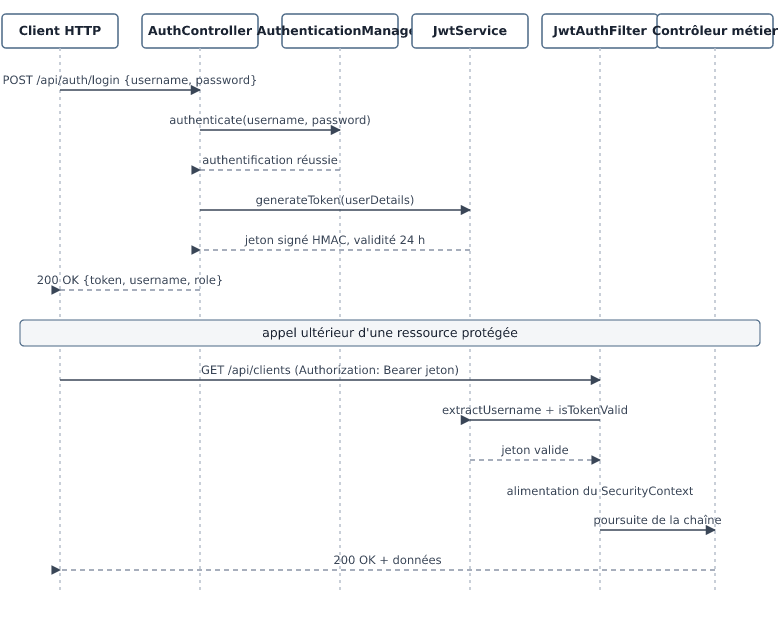
\includegraphics[width=0.95\linewidth]{figures/fig3.png}
\caption{Figure 3 — Séquence d'authentification et d'accès à une ressource protégée}
\end{figure}
Trois principes ont guidé cette conception. Les mots de passe sont \textbf{hachés avec BCrypt} avant persistance, algorithme intégrant un sel et un coût de calcul paramétrable. La politique de session est fixée à \textbf{`STATELESS`}, cohérente avec un service consommé par des clients hétérogènes. La protection \textbf{CSRF est désactivée}~: cette attaque exploite l'envoi automatique des cookies par le navigateur, mécanisme non utilisé ici puisque le jeton est transmis explicitement dans un en-tête. Ce choix est justifié dans le contexte d'une API sans cookie, mais devrait être réévalué si une authentification par cookie était introduite.
L'autorisation distingue deux rôles, \texttt{ADMIN} et \texttt{AGENT}. Elle a été conçue à deux niveaux~: par \textbf{chemin d'accès}, dans la configuration de la chaîne de filtres, et par \textbf{méthode}, au moyen d'annotations. Le second niveau n'a pas été activé, ce qui réduit la portée réelle du premier~; cette différence est analysée en sections 4.4 et 5.4, car elle constitue le principal défaut du travail.
\section*{3.5. Conception de l'API REST}
\addcontentsline{toc}{section}{3.5. Conception de l'API REST}
Les points d'accès suivent les conventions REST~: ressources désignées par des noms au pluriel, verbes HTTP porteurs de la sémantique de l'opération, codes de statut normalisés par la RFC 9110 [5] — 200 pour une lecture, 201 pour une création, 204 pour une suppression sans corps. La liste complète figure en annexe A.
Les sinistres sont exposés comme une \textbf{sous-ressource du contrat} (\texttt{/api/contracts/\{identifiant\}/claims}) et non seulement comme une ressource racine~: ce choix traduit dans l'URL la dépendance d'existence, l'identifiant du contrat devenant un paramètre obligatoire du chemin plutôt qu'un champ facultatif du corps de la requête. Enfin, la génération des identifiants métier — numéros de police et de sinistre — est \textbf{assumée par le serveur}, de même que la date de création d'un client, la date de déclaration d'un sinistre et le statut initial d'un contrat, ce qui évite qu'un client défectueux n'impose des valeurs incohérentes.
\section*{3.6. Environnement d'exécution conteneurisé}
\addcontentsline{toc}{section}{3.6. Environnement d'exécution conteneurisé}
Pour répondre au besoin de portabilité, l'application et sa base sont décrites sous forme de deux services conteneurisés orchestrés par Docker Compose (figure 4).
\begin{figure}[htbp]\centering
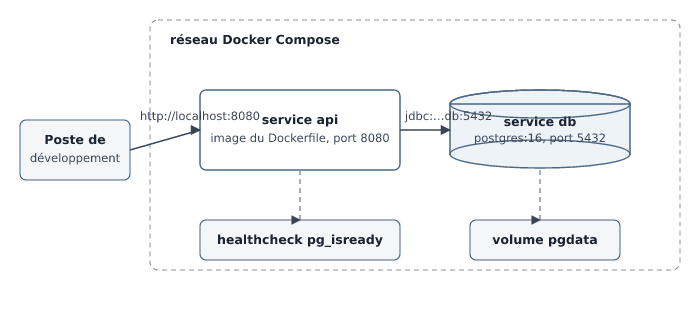
\includegraphics[width=0.95\linewidth]{figures/fig4.png}
\caption{Figure 4 — Composition de l'environnement Docker Compose}
\end{figure}
Deux mécanismes garantissent un démarrage fiable. Un \textbf{contrôle de santé} (\texttt{pg\_isready}) est défini sur le service de base de données, et le service applicatif déclare une dépendance conditionnée à ce contrôle~: l'API n'est lancée qu'une fois PostgreSQL réellement prêt à accepter des connexions, et non simplement démarré. Un \textbf{volume nommé} assure la persistance des données entre deux arrêts de la pile.
\textit{La conception étant établie, le chapitre suivant décrit sa traduction en code.}
\newpage
\chapter*{Chapitre 4 — Réalisation technique}
\addcontentsline{toc}{chapter}{Chapitre 4 — Réalisation technique}
\section*{4.1. Stack technique et justification des choix}
\addcontentsline{toc}{section}{4.1. Stack technique et justification des choix}
Le tableau 2 récapitule les composants retenus et la raison de chaque choix.
\begin{center}\textit{Tableau 2 — Stack technique et justification}\end{center}
{\small
\begin{tabularx}{\linewidth}{|X|X|X|}
\hline
\textbf{Composant} & \textbf{Version} & \textbf{Justification du choix} \\ \hline
Java & 17 & Version à support long~; introduit les \textit{records}, utilisés pour les DTO \\ \hline
Spring Boot & 3.5.16 & Auto-configuration, serveur embarqué~; socle utilisé par l'équipe d'accueil [9] \\ \hline
Spring Data JPA / Hibernate & héritées & Réduisent l'accès aux données à des déclarations d'interfaces [11] \\ \hline
PostgreSQL & 16 & Base relationnelle robuste et gratuite, adaptée aux contraintes d'intégrité [14] \\ \hline
Spring Security & héritée & Chaîne de filtres et infrastructure d'authentification [10] \\ \hline
JJWT & 0.12.6 & Bibliothèque de référence pour la manipulation de jetons en Java \\ \hline
Bean Validation & héritée & Validation déclarative par annotations sur les DTO \\ \hline
springdoc-openapi & 2.7.0 & Génère la spécification OpenAPI [12] et l'interface Swagger UI \\ \hline
Maven (wrapper) & 3.9.16 & Le wrapper garantit une version de build identique pour tous \\ \hline
Docker / Compose & — & Reproductibilité de l'environnement de développement [6] \\ \hline
Angular & 21.2 & Client web — initiative personnelle hors périmètre [13] \\ \hline
Chart.js & 4.5.1 & Graphique du tableau de bord du client web \\ \hline
\end{tabularx}

}
Le choix de Spring Boot n'était pas discutable~: il s'agit du socle utilisé par l'équipe d'accueil, et l'un des objectifs du stage était de me familiariser avec cet écosystème. L'ampleur du framework a néanmoins constitué une réelle difficulté d'apprentissage (section 5.3).
\section*{4.2. Mise en place du backend Spring Boot}
\addcontentsline{toc}{section}{4.2. Mise en place du backend Spring Boot}
Le projet a été initialisé avec Spring Initializr, puis structuré selon les paquetages décrits en section 3.3. L'injection de dépendances est réalisée \textbf{par constructeur} dans l'ensemble des classes, sans annotation sur les champs~: ce style rend les dépendances explicites, autorise la déclaration des champs en \texttt{final} et permet d'instancier une classe hors du conteneur Spring — condition nécessaire à l'écriture de tests unitaires avec des doublures. Les DTO sont implémentés sous forme de \textit{records} Java, immuables et dépourvus de code répétitif~:
\begin{verbatim}
public record ClientCreateDto(
        @NotBlank String lastName,
        @NotBlank String firstName,
        @Email @NotBlank String email,
        @NotBlank @Pattern(regexp = "\\d{8}",
            message = "Le CIN doit contenir exactement 8 chiffres") String cin,
        @NotBlank @Pattern(regexp = "\\d{8}",
            message = "Le téléphone doit contenir exactement 8 chiffres") String phoneNumber,
        @NotBlank String address,
        @NotNull LocalDate birthDate
) {}
\end{verbatim}
\begin{center}\textit{Extrait 1 — DTO de création d'un client. Les annotations de Bean Validation sont évaluées lorsque le paramètre du contrôleur est annoté \texttt{@Valid}~; une entrée invalide est rejetée avant d'atteindre la couche service. Les deux motifs à huit chiffres traduisent le format réel de la carte d'identité nationale et du numéro de téléphone tunisiens.}\end{center}
\section*{4.3. Persistance PostgreSQL et JPA}
\addcontentsline{toc}{section}{4.3. Persistance PostgreSQL et JPA}
Les quatre entités sont annotées \texttt{@Entity} et dotées d'un identifiant technique généré par la base. L'entité \texttt{User} est explicitement mappée sur la table \texttt{app\_user}, \texttt{user} étant un mot réservé en SQL [14]. Les contraintes d'intégrité sont déclarées au niveau du mapping et donc répercutées dans le schéma~: unicité du numéro d'identité nationale, du numéro de police, du numéro de sinistre, du nom d'utilisateur et du courriel~; non-nullité des champs obligatoires~; clés étrangères non nulles. Porter ces règles dans le schéma plutôt que dans le seul code garantit qu'elles restent valides même si une écriture contourne l'application.
Les \textit{repositories} étendent \texttt{JpaRepository}, ce qui fournit les opérations élémentaires sans code [11]. Huit méthodes ont été déclarées par dérivation à partir du nom~: \texttt{findByUsername} et \texttt{findByEmail} pour les utilisateurs, \texttt{existsByCin} et \texttt{findByActiveTrue} pour les clients, \texttt{findByClientId} et \texttt{existsByClientId} pour les contrats, \texttt{findByContractId} et \texttt{existsByContractId} pour les sinistres. Deux d'entre elles — \texttt{existsByClientId} et \texttt{existsByContractId} — sont déclarées mais \textbf{jamais appelées}~: la première devait servir au besoin BF5, resté inachevé.
Enfin, \texttt{open-in-view} est fixé à \texttt{false}. Cette propriété, activée par défaut, maintient la session Hibernate ouverte pendant le rendu de la réponse et masque ainsi les chargements paresseux involontaires~; la désactiver oblige à traiter explicitement les accès aux associations dans la couche service, ce qui évite des requêtes SQL non maîtrisées.
\section*{4.4. Authentification et autorisation}
\addcontentsline{toc}{section}{4.4. Authentification et autorisation}
\texttt{JwtService} centralise la manipulation des jetons~: génération avec le nom d'utilisateur comme sujet, date d'émission, expiration à vingt-quatre heures et signature HMAC~; puis extraction du sujet et vérification de validité. La clé est décodée depuis une chaîne Base64 lue dans la configuration.
\texttt{JwtAuthFilter} étend \texttt{OncePerRequestFilter} et s'intercale avant le filtre d'authentification par formulaire [10]~:
\begin{verbatim}
final String authHeader = request.getHeader("Authorization");
if (authHeader == null || !authHeader.startsWith("Bearer ")) {
    filterChain.doFilter(request, response);   // requête anonyme
    return;
}
final String jwt = authHeader.substring(7);
final String username = jwtService.extractUsername(jwt);

if (username != null && SecurityContextHolder.getContext().getAuthentication() == null) {
    UserDetails userDetails = userDetailsService.loadUserByUsername(username);
    if (jwtService.isTokenValid(jwt, userDetails)) {
        UsernamePasswordAuthenticationToken authToken =
                new UsernamePasswordAuthenticationToken(
                        userDetails, null, userDetails.getAuthorities());
        SecurityContextHolder.getContext().setAuthentication(authToken);
    }
}
filterChain.doFilter(request, response);
\end{verbatim}
\begin{center}\textit{Extrait 2 — Cœur du filtre d'authentification par jeton. Le filtre ne rejette jamais une requête lui-même~: il se contente de renseigner le contexte de sécurité, et c'est la chaîne configurée dans \texttt{SecurityConfig} qui décide ensuite d'autoriser ou de refuser l'accès.}\end{center}
Concernant l'\textbf{autorisation par rôle}, il convient d'être précis, car deux mécanismes coexistent avec des destins différents.
Le premier, \textbf{l'autorisation par chemin d'accès, est active}. La chaîne de filtres déclare explicitement que \texttt{/api/users/**} exige le rôle \texttt{ADMIN}, tandis que \texttt{/api/clients/**}, \texttt{/api/contracts/**} et \texttt{/api/claims/**} exigent \texttt{ADMIN} ou \texttt{AGENT}, et que toute autre requête exige une authentification. Un compte \texttt{AGENT} qui interroge la liste des employés reçoit donc bien un refus~: cette restriction fonctionne et a été vérifiée.
Le second, \textbf{l'autorisation par méthode, est inopérante}. Cinq annotations \texttt{@PreAuthorize} ont été posées sur des méthodes de contrôleur — restriction au rôle \texttt{ADMIN} pour la suppression d'un client et la modification d'un contrat, autorisation des deux rôles pour les trois lectures de sinistres — et une sixième a été laissée commentée. Or l'annotation d'activation \texttt{@EnableMethodSecurity} n'a jamais été ajoutée à la configuration. Ces annotations sont donc \textbf{présentes dans le code mais non appliquées à l'exécution}. La conséquence est concrète~: un compte \texttt{AGENT} peut supprimer un client et modifier un contrat, alors que la lecture du code laisse croire le contraire. Ce point est repris en section 5.4.
\section*{4.5. Fonctionnalités implémentées et règles métier}
\addcontentsline{toc}{section}{4.5. Fonctionnalités implémentées et règles métier}
Dix-sept points d'accès sont exposés, couvrant l'authentification, la gestion complète des clients, celle des contrats, la déclaration et la consultation des sinistres, et la consultation des employés (annexe A). La valeur de l'application ne réside toutefois pas dans ces opérations d'accès aux données, mais dans les règles que le serveur fait respecter (tableau 3).
\begin{center}\textit{Tableau 3 — Règles métier implémentées}\end{center}
{\small
\begin{tabularx}{\linewidth}{|X|X|X|X|}
\hline
\textbf{Réf.} & \textbf{Règle} & \textbf{Emplacement} & \textbf{Réaction} \\ \hline
RM1 & Le numéro d'identité nationale doit être unique & \texttt{ClientService} & Exception métier \\ \hline
RM2 & Le client doit avoir au moins 18 ans & \texttt{ClientService} & Exception métier \\ \hline
RM3 & La date de création d'un client est fixée par le serveur & \texttt{ClientService} & Valeur imposée \\ \hline
RM4 & Seuls les clients non archivés sont listés & \texttt{ClientService} & Filtrage \\ \hline
RM5 & Un client archivé ne peut plus être modifié & \texttt{ClientService} & Exception métier \\ \hline
RM6 & Le numéro d'identité nationale n'est pas modifiable & \texttt{ClientUpdateDto} & Absence structurelle \\ \hline
RM7 & La suppression d'un client est un archivage & \texttt{ClientService} & Valeur imposée \\ \hline
RM8 & Un contrat exige un client existant & \texttt{ContractService} & Exception métier \\ \hline
RM9 & La date de fin ne peut précéder la date de début & \texttt{ContractService} & Exception métier \\ \hline
RM10 & Un contrat créé est nécessairement \texttt{ACTIVE} & \texttt{ContractService} & Valeur imposée \\ \hline
RM11 & Le numéro de police est généré par le serveur & \texttt{ContractService} & Valeur imposée \\ \hline
RM12 & Un statut de contrat invalide est rejeté à la mise à jour & \texttt{ContractService} & Exception métier \\ \hline
RM13 & Aucun sinistre sur un contrat non \texttt{ACTIVE} & \texttt{ClaimService} & Exception métier \\ \hline
RM14 & La date de survenance doit tomber dans la période de couverture & \texttt{ClaimService} & Exception métier \\ \hline
RM15 & Un sinistre créé est \texttt{SUBMITTED}, remboursement à zéro & \texttt{ClaimService} & Valeurs imposées \\ \hline
RM16 & Le justificatif est renommé avant stockage & \texttt{ClaimService} & Identifiant unique \\ \hline
RM17 & Nom d'utilisateur et courriel sont uniques & \texttt{UserService} & Exception \\ \hline
RM18 & Le mot de passe est haché avant persistance & \texttt{UserService} & BCrypt \\ \hline
\end{tabularx}

}
La règle RM13 illustre la logique du domaine~: accepter une déclaration de sinistre sur un contrat résilié ou expiré créerait une donnée dépourvue de sens juridique. Le contrôle est placé dans la couche service, ce qui garantit son application quel que soit le point d'entrée.
\begin{verbatim}
@Transactional
public ClaimResponseDto createClaim(Long contractId, ClaimCreateDto dto,
                                    MultipartFile file) {
    Contract contract = contractRepository.findById(contractId)
            .orElseThrow(() -> new NotFoundException(
                    "Contract not found with ID: " + contractId));

    if (contract.getStatus() != ContractStatus.ACTIVE) {
        throw new BusinessRuleException(
                "Cannot file a claim: Contract is not ACTIVE");
    }
    if (dto.claimDate().isBefore(contract.getStartDate())
            || dto.claimDate().isAfter(contract.getEndDate())) {
        throw new BusinessRuleException(
                "Claim date must be within the contract coverage period");
    }
    // statut SUBMITTED, remboursement à zéro, numéro généré,
    // justificatif renommé puis persisté
}
\end{verbatim}
\begin{center}\textit{Extrait 3 — Application des règles RM13 et RM14. La méthode est transactionnelle~: en cas d'exception, aucune écriture partielle n'est validée. Le troisième paramètre transporte le justificatif téléversé.}\end{center}
La déclaration d'un sinistre accepte en effet un \textbf{justificatif facultatif}, transmis en \texttt{multipart/form-data}. Le fichier est renommé avec un identifiant unique afin d'éviter tout écrasement, conservé dans un dossier \texttt{uploads}, et son chemin est enregistré en base. Aucun point d'accès de restitution n'a été prévu dans le temps du stage.
Un composant \texttt{DataInitializer} alimente la base au démarrage si elle est vide~: deux comptes utilisateurs — un administrateur et un agent —, un client et deux contrats, l'un actif et l'autre résilié, ce dernier permettant de vérifier immédiatement la règle RM13. Il s'agit exclusivement de \textbf{données de démonstration destinées au développement local}~; elles n'ont pas vocation à exister dans un environnement réel et devraient être conditionnées à un profil Spring dédié.
\section*{4.6. Documentation OpenAPI}
\addcontentsline{toc}{section}{4.6. Documentation OpenAPI}
La dépendance \texttt{springdoc-openapi} génère automatiquement la spécification OpenAPI [12] à partir des signatures des contrôleurs et l'expose via une interface Swagger UI. Une classe de configuration complète cette génération en déclarant le titre, la version et surtout un schéma de sécurité \texttt{bearerAuth} appliqué à l'ensemble des routes. L'intérêt pratique est immédiat~: le bouton « Authorize » permet de coller le jeton obtenu au \textit{login} puis de tester toutes les routes protégées depuis le navigateur, sans outil externe. Pendant le développement, cette documentation a servi d'outil de test principal.
\section*{4.7. Conteneurisation avec Docker Compose}
\addcontentsline{toc}{section}{4.7. Conteneurisation avec Docker Compose}
Le \texttt{Dockerfile} est construit en \textbf{deux étapes}. La première utilise une image contenant Maven et le JDK 17 pour compiler le projet et produire une archive exécutable~; la seconde repart d'une image ne contenant qu'un environnement d'exécution Java et n'y copie que l'archive produite. Cette construction en plusieurs étapes est la pratique recommandée par la documentation Docker [6]~: l'image finale ne contient ni code source, ni Maven, ni cache de dépendances, ce qui réduit sa taille et sa surface d'exposition.
La configuration de l'API est injectée par variables d'environnement, que le fichier de configuration consomme via des valeurs par défaut surchargeables. La même image fonctionne donc en local et en conteneur sans modification de code — application directe du principe de configuration externalisée [7]. Le résultat est un \textbf{environnement de développement reproductible}~: deux commandes suffisent à démarrer l'API et sa base sur un poste vierge. Il ne s'agit pas d'un dispositif de production~; les limites sont détaillées en section 5.4.
\section*{4.8. Initiative personnelle~: client web Angular}
\addcontentsline{toc}{section}{4.8. Initiative personnelle~: client web Angular}
Cette section décrit un travail \textbf{non demandé par l'entreprise}, mené en fin de stage à titre d'apprentissage~: découvrir Angular [13] et valider en conditions réelles que l'API était consommable par un client navigateur — ce qui met à l'épreuve la configuration CORS et la transmission du jeton.
\begin{figure}[htbp]\centering
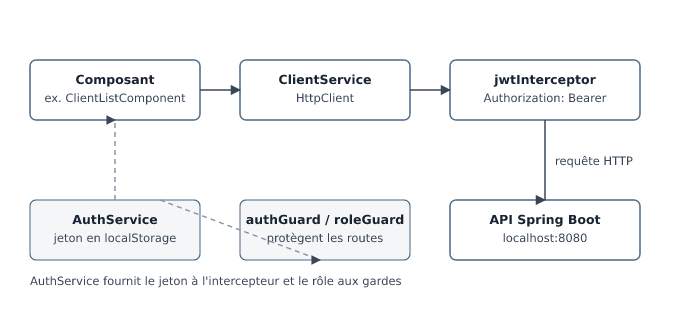
\includegraphics[width=0.95\linewidth]{figures/fig5.png}
\caption{Figure 5 — Chaîne d'appel du client web Angular vers l'API}
\end{figure}
Trois pièces constituent le mécanisme d'authentification côté client (figure 5). Un \textbf{service d'authentification} appelle la route de connexion et conserve le jeton dans le stockage local du navigateur. Un \textbf{intercepteur HTTP} ajoute automatiquement l'en-tête \texttt{Authorization} à chaque requête sortante, évitant de répéter cette logique dans chaque service. Une \textbf{garde de route} empêche l'accès aux pages protégées en l'absence de jeton. Une seconde garde, fondée sur le rôle, complète ce dispositif~: la page de gestion des employés et son lien de navigation ne sont accessibles qu'à un administrateur, ce qui double côté client la restriction que le backend applique sur \texttt{/api/users/**}. L'état des composants est géré par \textbf{signaux}, mécanisme réactif natif d'Angular, et le tableau de bord agrège trois compteurs dans un graphique en barres.
Onze écrans ont été réalisés~: connexion, tableau de bord, liste et fiche des clients, formulaire de création d'un client, liste et détail des contrats, liste, déclaration et détail des sinistres, et gestion des employés. Le formulaire de déclaration de sinistre enchaîne la sélection d'un client puis de l'un de ses contrats, et transmet le justificatif au format \texttt{multipart/form-data}.
L'état d'avancement doit être présenté sans exagération. Quatre opérations exposées par l'API \textbf{ne sont pas accessibles depuis l'interface}~: la modification et l'archivage d'un client, la création et la modification d'un contrat — elles restent testables via Swagger. L'URL de l'API est codée en dur dans les cinq services~; l'intercepteur ne traite pas les réponses 401, si bien qu'un jeton expiré n'entraîne pas de redirection~; aucun formulaire n'est validé côté client, les règles de format n'étant découvertes qu'après l'appel réseau~; le jeton est conservé dans le stockage local, ce qui l'expose aux injections de script. Surtout, \textbf{la suite de tests générée par l'outil de construction n'a jamais été adaptée}~: huit des neuf fichiers de test référencent des noms de classes inexistants et la suite ne compile pas. Ce client web est donc une \textbf{maquette d'apprentissage}, utile comme preuve de consommation de l'API, et non un produit livrable.
\textit{Le chapitre suivant expose la manière dont ces développements ont été vérifiés et les limites du travail réalisé.}
\newpage
\chapter*{Chapitre 5 — Vérification, résultats et regard critique}
\addcontentsline{toc}{chapter}{Chapitre 5 — Vérification, résultats et regard critique}
\section*{5.1. Stratégie de vérification}
\addcontentsline{toc}{section}{5.1. Stratégie de vérification}
La vérification a reposé sur trois moyens d'importance inégale.
Les \textbf{tests automatisés backend} sont au nombre de deux. Le premier vérifie que le contexte Spring démarre correctement~: il détecte les erreurs de configuration, mais requiert une base PostgreSQL accessible, ce qui le rend dépendant de l'environnement. Le second est un test unitaire écrit avec JUnit 5 et Mockito~: il simule un contrat au statut \texttt{TERMINATED} et vérifie que la déclaration d'un sinistre lève bien une exception métier. Il valide la règle RM13, la plus caractéristique du domaine, et n'a été rendu possible que par l'injection par constructeur, qui permet d'instancier le service avec des \textit{repositories} simulés.
Les \textbf{tests manuels via Swagger UI} ont constitué l'outil de vérification principal au quotidien~: après chaque nouvelle fonctionnalité, le parcours complet — authentification, création d'un client, création d'un contrat, déclaration d'un sinistre — était rejoué depuis le navigateur. Les \textbf{vérifications en base} avec \texttt{psql} ont permis de contrôler que le schéma généré portait bien les contraintes attendues. Côté client web, la compilation du projet a été vérifiée et le parcours de connexion, de consultation et de création rejoué dans le navigateur.
La limite doit être énoncée clairement~: \textbf{la couverture de test automatisée est très faible}. Un seul test unitaire couvre une seule des dix-huit règles métier du tableau 3~; aucun test de contrôleur, de sécurité ou d'intégration n'a été écrit~; la suite de tests du client web ne compile pas~; aucun taux de couverture n'est mesuré, faute d'outil de mesure dans la configuration de build.
\section*{5.2. Résultats obtenus}
\addcontentsline{toc}{section}{5.2. Résultats obtenus}
L'API est fonctionnelle sur l'ensemble des besoins retenus au tableau 1, à l'exception de BF5, inachevé, et de BF12, explicitement reporté. Les vérifications confirment les comportements suivants~:
\begin{itemize}\item une requête sans jeton sur une route métier est rejetée~;\end{itemize}
\begin{itemize}\item une connexion valide renvoie un jeton exploitable pendant vingt-quatre heures, accompagné du nom d'utilisateur et du rôle~;\end{itemize}
\begin{itemize}\item une déclaration de sinistre sur le contrat résilié du jeu de démonstration est refusée avec un message explicite, de même qu'une déclaration hors période de couverture~;\end{itemize}
\begin{itemize}\item un client mineur, un numéro d'identité nationale déjà utilisé, un courriel malformé ou un numéro de téléphone qui ne compte pas huit chiffres sont rejetés avant d'atteindre la couche service~;\end{itemize}
\begin{itemize}\item un client créé reçoit une date de création serveur et un contrat un numéro de police généré~;\end{itemize}
\begin{itemize}\item l'archivage d'un client le fait disparaître de la liste sans supprimer ses contrats~;\end{itemize}
\begin{itemize}\item un compte \texttt{AGENT} qui interroge la liste des employés reçoit un refus, tandis qu'un compte \texttt{ADMIN} y accède~;\end{itemize}
\begin{itemize}\item la pile Docker Compose démarre la base puis l'API dans cet ordre~;\end{itemize}
\begin{itemize}\item le client web parvient à s'authentifier, à afficher les clients, les contrats et les sinistres, à créer un client et à déclarer un sinistre avec justificatif.\end{itemize}
\section*{5.3. Difficultés rencontrées et solutions}
\addcontentsline{toc}{section}{5.3. Difficultés rencontrées et solutions}
Huit difficultés significatives ont jalonné le développement. Le tableau 4 en donne l'analyse et la solution retenue.
\begin{center}\textit{Tableau 4 — Difficultés rencontrées et solutions apportées}\end{center}
{\small
\begin{tabularx}{\linewidth}{|X|X|X|}
\hline
\textbf{Difficulté} & \textbf{Analyse} & \textbf{Solution retenue} \\ \hline
Échec au démarrage sur la table \texttt{user} & \texttt{user} est un mot réservé de SQL & Mappage explicite sur la table \texttt{app\_user} \\ \hline
\texttt{LazyInitializationException} à la sérialisation & Associations \texttt{LAZY} accédées hors transaction, \texttt{open-in-view} désactivé & Conversion en DTO dans les méthodes \texttt{@Transactional} \\ \hline
Requêtes du navigateur bloquées & Politique de même origine entre les ports 4200 et 8080 & Déclaration d'une source de configuration CORS et activation dans la chaîne \\ \hline
Ordre de démarrage des conteneurs & L'API démarrait avant que PostgreSQL n'accepte les connexions & Contrôle de santé \texttt{pg\_isready} et dépendance conditionnée \\ \hline
Configuration figée entre local et conteneur & L'URL de la base différait selon le contexte & Externalisation par variables d'environnement avec valeurs par défaut \\ \hline
Entités exposées directement & Les premières versions divulguaient des champs internes & Introduction de DTO dédiés et de classes de conversion \\ \hline
Envoi du justificatif refusé & Un corps JSON ne peut pas transporter un fichier binaire & Passage en \texttt{multipart/form-data} et liaison par \texttt{@ModelAttribute} au lieu de \texttt{@RequestBody} \\ \hline
Courbe d'apprentissage de Spring Security & Le fonctionnement de la chaîne de filtres n'était pas intuitif & Lecture de la documentation de référence [10], puis reconstruction pas à pas du filtre \\ \hline
\end{tabularx}

}
La difficulté relative au chargement paresseux a été la plus formatrice. Elle m'a obligé à comprendre que le cycle de vie d'un objet JPA est lié à celui de la transaction, notion que je n'avais abordée que théoriquement en cours. La désactivation d'\texttt{open-in-view} n'a pas causé le problème~: elle l'a rendu visible au lieu de le masquer derrière des requêtes SQL émises silencieusement.
Le passage au \texttt{multipart/form-data} a eu un effet de bord que je n'ai identifié qu'après coup~: la liaison par \texttt{@ModelAttribute} ne déclenche pas la validation Bean Validation de la même manière que \texttt{@RequestBody} annoté de \texttt{@Valid}. Les contraintes portées par le DTO de sinistre ne sont donc pas évaluées sur cette route, ce qui constitue une régression discrète — exactement le type de défaut qu'un test de contrôleur aurait détecté.
\section*{5.4. Regard critique et limites}
\addcontentsline{toc}{section}{5.4. Regard critique et limites}
Le socle produit me paraît correct sur le plan structurel~: responsabilités séparées, règles métier centralisées côté serveur, contraintes d'intégrité portées par le schéma, interface documentée. Plusieurs faiblesses doivent néanmoins être reconnues.
\textbf{L'autorisation par méthode n'est pas effective.} C'est le défaut le plus important. Les cinq annotations \texttt{@PreAuthorize} sont inopérantes faute d'activation de la sécurité au niveau des méthodes~: tout utilisateur authentifié, y compris un compte \texttt{AGENT}, peut archiver un client ou modifier un contrat. La restriction par chemin d'accès, elle, fonctionne — la liste des employés est bien réservée à l'administrateur — mais elle ne couvre pas les opérations sensibles des autres ressources. Une annotation qui donne l'illusion d'une protection est plus dangereuse qu'une absence de protection assumée, car elle trompe le lecteur du code. La correction est brève~: activer la sécurité au niveau des méthodes, puis écrire les tests vérifiant effectivement les refus.
\textbf{Une règle annoncée n'est pas implémentée.} Le besoin BF5 — interdire l'archivage d'un client encore rattaché à un contrat — dispose de sa méthode de vérification dans la couche d'accès aux données, mais celle-ci n'est jamais appelée~: le dépôt de contrats est injecté dans le service client sans être utilisé. Un client porteur de contrats peut donc être archivé, et ses contrats continuent d'apparaître dans les listes. J'ai choisi de documenter cet écart plutôt que de le corriger dans l'urgence en fin de stage, parce qu'un contrôle non testé aurait ajouté une fausse garantie à une autre.
\textbf{La gestion des erreurs est trop grossière.} Le gestionnaire global intercepte toute exception d'exécution et renvoie systématiquement un statut 400. Une ressource inexistante devrait produire un 404, une violation de règle métier un 409 ou un 422, un échec d'authentification un 401, un accès refusé un 403~; en l'état, le client ne peut pas distinguer ces situations. Il faudrait des gestionnaires par type d'exception et un format d'erreur normalisé [8].
\textbf{Le secret de signature des jetons est en clair dans le dépôt.} La propriété correspondante est écrite en dur dans le fichier de configuration, contrairement aux paramètres de base de données qui sont, eux, externalisés. Il s'agit d'un secret de développement, mais l'habitude prise est mauvaise~: une injection par variable d'environnement s'impose.
\textbf{Le schéma est géré automatiquement par Hibernate.} Le mode \texttt{ddl-auto: update} est pratique en développement mais inadapté dès qu'il existe des données à préserver~: il n'exécute aucune suppression ni renommage, ne trace pas les évolutions et ne permet pas de revenir en arrière.
\textbf{Le jeton est peu défensif.} Il ne porte pas le rôle en revendication, sa validité de vingt-quatre heures est longue, il n'existe ni rafraîchissement ni révocation, et le filtre ne capture pas les exceptions d'analyse~: un jeton expiré ou malformé provoque une remontée d'exception plutôt qu'une réponse 401 propre.
\textbf{Le téléversement de justificatifs n'est pas durci.} Aucune limite de taille n'est configurée, aucun type de fichier n'est contrôlé, et le dossier de destination n'est pas monté en volume dans l'environnement conteneurisé~: les documents seraient perdus à la recréation du conteneur. Deux fichiers de démonstration ont d'ailleurs été commités par accident, la règle d'exclusion du dépôt ayant été écrite dans un encodage de caractères que Git ne reconnaît pas.
\textbf{La conteneurisation reste orientée développement.} L'image s'exécute avec l'utilisateur \texttt{root}, les identifiants figurent en clair dans le fichier de composition, aucune limite de ressources n'est fixée, les dépendances Maven ne sont pas mises en cache et les tests sont ignorés lors de la construction. L'objectif visé — la reproductibilité en développement — est atteint~; l'objectif « production » ne l'est pas et n'était pas visé.
Trois faiblesses complètent ce constat. \textbf{Aucune intégration continue n'est en place}~: rien ne garantit automatiquement que le projet compile et que les tests passent avant une fusion. \textbf{L'API manque de robustesse à l'échelle}~: les listes sont renvoyées intégralement, sans pagination ni filtre, et le client web en profite pour filtrer côté navigateur des données qu'une route dédiée aurait pu restituer directement. \textbf{La documentation du dépôt est en retard sur le code}~: le \texttt{README.md} annonce une gestion des clients limitée à la création et à la lecture alors que la modification et l'archivage existent, ne mentionne qu'un seul des deux comptes de démonstration, et ne parle ni de Docker, ni du téléversement, ni du client web~; le diagramme de classes du dossier \texttt{docs} omet le booléen d'archivage et le chemin du justificatif.
\textit{Ces constats, y compris les plus défavorables, constituent l'essentiel de ce que ce stage m'a appris~; le chapitre suivant en tire le bilan.}
\newpage
\chapter*{Chapitre 6 — Apports du stage et lien avec la formation}
\addcontentsline{toc}{chapter}{Chapitre 6 — Apports du stage et lien avec la formation}
\section*{6.1. Compétences techniques acquises}
\addcontentsline{toc}{section}{6.1. Compétences techniques acquises}
\begin{center}\textit{Tableau 5 — Compétences acquises et modules associés}\end{center}
{\small
\begin{tabularx}{\linewidth}{|X|X|X|}
\hline
\textbf{Compétence} & \textbf{Niveau atteint} & \textbf{Module associé} \\ \hline
Programmation orientée objet en Java 17 & Consolidé & Programmation orientée objet \\ \hline
Conception relationnelle et contraintes d'intégrité & Consolidé & Bases de données \\ \hline
Mappage objet-relationnel avec JPA et Hibernate & Nouveau & Bases de données (prolongement) \\ \hline
Développement d'une API REST avec Spring Boot & Nouveau & Programmation web (prolongement) \\ \hline
Architecture en couches et séparation des responsabilités & Nouveau & Génie logiciel \\ \hline
Authentification par jeton et hachage de mots de passe & Nouveau & Sécurité informatique (notions) \\ \hline
Test unitaire avec JUnit 5 et Mockito & Initié & Génie logiciel \\ \hline
Conteneurisation avec Docker et Docker Compose & Nouveau & Systèmes d'exploitation (prolongement) \\ \hline
Gestion de versions avec Git et branches & Consolidé & Outils de développement \\ \hline
Développement d'un client Angular (composants autonomes, signaux, guards, intercepteurs) & Initié — hors périmètre & Programmation web \\ \hline
\end{tabularx}

}
Au-delà de la liste, trois acquis me paraissent structurants. D'abord, la compréhension du \textbf{rôle du serveur comme garant des règles métier}~: avant ce stage, j'aurais volontiers laissé le client vérifier qu'une date de sinistre tombe dans la période de couverture. Ensuite, la notion de \textbf{contrat d'interface}~: distinguer ce qu'une API accepte, ce qu'elle renvoie et ce qu'elle stocke est une discipline que je n'appliquais pas. Enfin, la \textbf{reproductibilité de l'environnement}~: constater qu'un projet démarre sur une machine vierge en deux commandes change la perception de ce qu'est un livrable.
\section*{6.2. Compétences transversales et lien avec la formation}
\addcontentsline{toc}{section}{6.2. Compétences transversales et lien avec la formation}
L'\textbf{autonomie} a été la première exigence~: sur un sujet largement nouveau, j'ai dû identifier moi-même les ressources pertinentes et distinguer une documentation officielle d'un tutoriel obsolète — plusieurs exemples de code trouvés en ligne s'appuyaient sur des interfaces de manipulation de jetons dépréciées. La \textbf{méthode de résolution de problèmes} a progressé~: l'erreur de chargement paresseux m'a appris à remonter à la cause première plutôt qu'à modifier le code au hasard jusqu'à la disparition du symptôme. La \textbf{rigueur documentaire} s'est développée par la pratique des messages de commit conventionnels et par la rédaction de ce rapport, qui m'a contraint à justifier chaque choix technique — exercice ayant révélé certaines des faiblesses exposées en section 5.4, notamment l'écart entre les annotations d'autorisation et leur effet réel. La \textbf{communication professionnelle} s'est exercée lors des points de validation~: présenter un avancement de façon synthétique, admettre ce qui ne fonctionne pas et poser une question précise sont des compétences que le cadre académique sollicite peu.
Le stage a prolongé plusieurs enseignements de première année. La \textbf{programmation orientée objet} a trouvé une application directe dans la modélisation des entités, l'encapsulation et l'usage des énumérations. Les \textbf{bases de données} se sont traduites par la conception du schéma, les contraintes d'unicité et de clé étrangère et la notion de transaction — cette dernière prenant, dans le contexte JPA, une dimension bien plus concrète qu'en cours. L'\textbf{algorithmique} a servi dans la structuration des traitements de service. Réciproquement, le stage a mis en évidence des domaines que la formation aborde plus tard~: architectures applicatives, sécurité des applications web, tests automatisés et déploiement. Cette découverte anticipée me permettra d'aborder ces modules avec un référentiel concret.
\section*{6.3. Limites personnelles et perspectives}
\addcontentsline{toc}{section}{6.3. Limites personnelles et perspectives}
Je reconnais trois limites personnelles. La \textbf{culture du test} m'a manqué~: j'ai écrit le code puis, tardivement, un unique test, au lieu de tester au fil des règles métier — et j'ai laissé se dégrader la suite de tests du client web sans la réparer. La \textbf{gestion du temps} a été imparfaite~: le temps consacré au client web, bien qu'instructif, aurait été mieux investi dans la correction de l'autorisation par méthode, du besoin BF5 et de la gestion des erreurs, trois défauts du périmètre effectivement demandé. Enfin, ma \textbf{maîtrise de Spring Security} reste superficielle~: je sais faire fonctionner la chaîne, je n'ai pas su diagnostiquer plus tôt l'absence d'activation de la sécurité au niveau des méthodes.
\begin{center}\textit{Tableau 6 — Limites identifiées et pistes d'amélioration}\end{center}
{\small
\begin{tabularx}{\linewidth}{|X|X|X|}
\hline
\textbf{Limite} & \textbf{Amélioration proposée} & \textbf{Effort} \\ \hline
Autorisation par méthode inopérante & Activer \texttt{@EnableMethodSecurity} et écrire les tests de refus par rôle & Faible \\ \hline
Besoin BF5 non implémenté & Brancher \texttt{existsByClientId} sur l'archivage et tester le refus & Faible \\ \hline
Erreurs toujours renvoyées en 400 & Gestionnaires par type d'exception, format RFC 9457 [8] & Faible \\ \hline
Secret de signature en dur & Injection par variable d'environnement & Faible \\ \hline
Validation absente sur la route de sinistre & Rétablir la validation explicite du DTO en \texttt{multipart} & Faible \\ \hline
Documentation du dépôt désalignée & Mise à jour du \texttt{README} et du diagramme de classes & Faible \\ \hline
Suite de tests du client web cassée & Réparer les huit fichiers de test et compléter la feuille de style tronquée & Faible \\ \hline
Téléversement non durci & Limite de taille, contrôle de type, volume persistant, restitution & Moyen \\ \hline
Couverture de test insuffisante & Tests de contrôleur et tests d'intégration sur base jetable, mesure de couverture & Moyen \\ \hline
Absence d'intégration continue & Chaîne automatisée~: compilation et tests à chaque poussée & Moyen \\ \hline
Schéma non versionné & Migrations versionnées avec un outil dédié & Moyen \\ \hline
Listes sans pagination & Pagination, tri et filtrage des ressources & Moyen \\ \hline
Workflow des sinistres absent & Modélisation des transitions de statut et du remboursement & Élevé \\ \hline
\end{tabularx}

}
\newpage
\chapter*{Conclusion}
\addcontentsline{toc}{chapter}{Conclusion}
Ce stage d'initiation d'un mois chez Vermeg avait pour objet la réalisation d'une mini-API REST de gestion d'assurance. L'objectif est atteint sur le périmètre demandé~: le service expose dix-sept points d'accès couvrant la gestion des clients, des contrats et des sinistres ainsi que la consultation des employés, s'appuie sur une base PostgreSQL, protège ses accès par un jeton, valide ses entrées, centralise dix-huit règles métier dans la couche service et publie une documentation OpenAPI interactive. La conteneurisation ajoutée en fin de parcours rend l'environnement de développement reproductible sur un poste tiers.
Sur le plan technique, j'ai découvert et pratiqué un écosystème que je ne connaissais pas — Spring Boot, JPA, Spring Security, Docker — et j'ai surtout compris pourquoi une architecture en couches, des objets de transfert dédiés et des règles métier centralisées côté serveur ne sont pas des raffinements théoriques mais des réponses à des problèmes concrets.
Sur le plan critique, le travail comporte des faiblesses que j'ai identifiées et documentées sans les minimiser~: une autorisation par méthode annotée mais non activée, un besoin annoncé mais non implémenté, une gestion des erreurs trop uniforme, une couverture de test très faible, un secret non externalisé, un téléversement non durci et une conteneurisation qui ne vise pas la production. Ces constats ont plus de valeur pédagogique que la liste des fonctionnalités livrées, car ils dessinent précisément ce que j'ai à travailler. Le client web développé en parallèle relève, quant à lui, d'une démarche personnelle de montée en compétences~: partiel, non testé et non demandé, il a néanmoins prouvé que l'API est consommable par un client réel.
Enfin, ce stage m'a donné un premier aperçu du fonctionnement d'une entreprise d'édition logicielle spécialisée, où la correction fonctionnelle, la traçabilité et la lisibilité du code comptent autant que le résultat visible. C'est cette exigence que je souhaite conserver pour la suite de mon cursus.
\newpage
\chapter*{Bibliographie et webographie}
\addcontentsline{toc}{chapter}{Bibliographie et webographie}
[1] VERMEG, « À propos — éditeur de solutions logicielles pour les services financiers ». [En ligne]. Disponible~: https://www.vermeg.com — consulté le 27 juillet 2026.
[2] Wikipedia, « Vermeg ». [En ligne]. Disponible~: https://en.wikipedia.org/wiki/Vermeg — consulté le 27 juillet 2026.
[3] Conventional Commits, « Conventional Commits 1.0.0 ». [En ligne]. Disponible~: https://www.conventionalcommits.org/fr/v1.0.0/ — consulté le 27 juillet 2026.
[4] M. JONES, J. BRADLEY et N. SAKIMURA, « RFC 7519~: JSON Web Token (JWT) », IETF, mai 2015. [En ligne]. Disponible~: https://www.rfc-editor.org/rfc/rfc7519
[5] R. FIELDING, M. NOTTINGHAM et J. RESCHKE, « RFC 9110~: HTTP Semantics », IETF, juin 2022. [En ligne]. Disponible~: https://www.rfc-editor.org/rfc/rfc9110
[6] Docker Inc., « Multi-stage builds », Docker Documentation. [En ligne]. Disponible~: https://docs.docker.com/build/building/multi-stage/ — consulté le 27 juillet 2026.
[7] A. WIGGINS, « The Twelve-Factor App — III. Config ». [En ligne]. Disponible~: https://12factor.net/fr/config — consulté le 27 juillet 2026.
[8] M. NOTTINGHAM, E. WILDE et S. DALAL, « RFC 9457~: Problem Details for HTTP APIs », IETF, juillet 2023. [En ligne]. Disponible~: https://www.rfc-editor.org/rfc/rfc9457
[9] VMware Tanzu, « Spring Boot Reference Documentation », version 3.5. [En ligne]. Disponible~: https://docs.spring.io/spring-boot/documentation.html — consulté le 27 juillet 2026.
[10] VMware Tanzu, « Spring Security Reference — Architecture ». [En ligne]. Disponible~: https://docs.spring.io/spring-security/reference/servlet/architecture.html — consulté le 27 juillet 2026.
[11] VMware Tanzu, « Spring Data JPA Reference Documentation ». [En ligne]. Disponible~: https://docs.spring.io/spring-data/jpa/reference/ — consulté le 27 juillet 2026.
[12] OpenAPI Initiative, « OpenAPI Specification v3.1 ». [En ligne]. Disponible~: https://spec.openapis.org/oas/v3.1.0 — consulté le 27 juillet 2026.
[13] Google, « Angular Documentation ». [En ligne]. Disponible~: https://angular.dev — consulté le 27 juillet 2026.
[14] The PostgreSQL Global Development Group, « PostgreSQL 16 Documentation ». [En ligne]. Disponible~: https://www.postgresql.org/docs/16/ — consulté le 27 juillet 2026.
\newpage
\chapter*{Annexe A — Points d'accès de l'API}
\addcontentsline{toc}{chapter}{Annexe A — Points d'accès de l'API}
\begin{center}\textit{Tableau A.1 — Inventaire des dix-sept points d'accès}\end{center}
{\small
\begin{tabularx}{\linewidth}{|X|X|X|X|X|X|}
\hline
\textbf{Méthode} & \textbf{Chemin} & \textbf{Corps de requête} & \textbf{Réponse} & \textbf{Statut} & \textbf{Accès} \\ \hline
POST & \texttt{/api/auth/register} & \texttt{\{username, password, role, firstName, lastName, email\}} & message & 201 & public \\ \hline
POST & \texttt{/api/auth/login} & \texttt{\{username, password\}} & \texttt{\{token, username, role\}} & 200 & public \\ \hline
POST & \texttt{/api/clients} & \texttt{ClientCreateDto} & \texttt{ClientResponseDto} & 201 & ADMIN, AGENT \\ \hline
GET & \texttt{/api/clients} & — & liste des clients non archivés & 200 & ADMIN, AGENT \\ \hline
GET & \texttt{/api/clients/\{id\}} & — & \texttt{ClientResponseDto} & 200 & ADMIN, AGENT \\ \hline
PUT & \texttt{/api/clients/\{id\}} & \texttt{ClientUpdateDto} & \texttt{ClientResponseDto} & 200 & ADMIN, AGENT \\ \hline
DELETE & \texttt{/api/clients/\{id\}} & — & — & 204 & ADMIN, AGENT \\ \hline
POST & \texttt{/api/contracts} & \texttt{ContractCreateDto} & \texttt{ContractResponseDto} & 201 & ADMIN, AGENT \\ \hline
GET & \texttt{/api/contracts} & — & liste de contrats & 200 & ADMIN, AGENT \\ \hline
GET & \texttt{/api/contracts/\{id\}} & — & \texttt{ContractResponseDto} & 200 & ADMIN, AGENT \\ \hline
PUT & \texttt{/api/contracts/\{id\}} & \texttt{ContractUpdateDto} & \texttt{ContractResponseDto} & 200 & ADMIN, AGENT \\ \hline
GET & \texttt{/api/contracts/client/\{clientId\}} & — & liste de contrats & 200 & ADMIN, AGENT \\ \hline
POST & \texttt{/api/contracts/\{contractId\}/claims} & \texttt{multipart/form-data}~: champs du DTO et justificatif facultatif & \texttt{ClaimResponseDto} & 201 & ADMIN, AGENT \\ \hline
GET & \texttt{/api/contracts/\{contractId\}/claims} & — & liste de sinistres & 200 & ADMIN, AGENT \\ \hline
GET & \texttt{/api/claims} & — & liste de sinistres & 200 & ADMIN, AGENT \\ \hline
GET & \texttt{/api/claims/\{id\}} & — & \texttt{ClaimResponseDto} & 200 & ADMIN, AGENT \\ \hline
GET & \texttt{/api/users} & — & liste des employés & 200 & ADMIN \\ \hline
\end{tabularx}

}
Toutes les routes, hormis \texttt{/api/auth/**}, \texttt{/swagger-ui/**} et \texttt{/v3/api-docs/**}, exigent un en-tête \texttt{Authorization: Bearer <jeton>}. La colonne « Accès » décrit la restriction effectivement appliquée par la chaîne de filtres~; les annotations posées sur les méthodes ne sont pas actives (section 4.4).
Exemple de corps de création d'un contrat~:
\begin{verbatim}
{ "clientId": 1, "type": "AUTO", "startDate": "2026-07-01",
  "endDate": "2027-06-30", "coverageAmount": 50000, "premiumAmount": 1200 }
\end{verbatim}
\chapter*{Annexe B — Instructions de démarrage}
\addcontentsline{toc}{chapter}{Annexe B — Instructions de démarrage}
\textbf{Exécution locale}
\begin{verbatim}
createdb assurance_db
export SPRING_DATASOURCE_URL=jdbc:postgresql://localhost:5432/assurance_db
export SPRING_DATASOURCE_USERNAME=postgres
export SPRING_DATASOURCE_PASSWORD=admin
./mvnw spring-boot:run
\end{verbatim}
\textbf{Exécution conteneurisée}
\begin{verbatim}
docker compose up --build   # démarre le service db puis le service api
docker compose down         # arrêt (le volume pgdata conserve les données)
docker compose down -v      # arrêt avec suppression des données
\end{verbatim}
\textbf{Accès} — Documentation interactive~: \texttt{http://localhost:8080/swagger-ui/index.html}. Client web optionnel~: \texttt{cd frontend \&\& npm ci \&\& npm start}, puis \texttt{http://localhost:4200}.
\textbf{Comptes de démonstration} — créés automatiquement au démarrage \textbf{à des fins de développement local uniquement}~: \texttt{admin} / \texttt{admin123} (rôle ADMIN) et \texttt{agent} / \texttt{agent123} (rôle AGENT). Ces identifiants n'ont aucune valeur hors du poste de développement et doivent être supprimés de tout environnement partagé.
\textbf{Tests} — \texttt{./mvnw test} (le test de contexte nécessite une base PostgreSQL accessible). La suite de tests du client web ne compile pas en l'état (section 4.8).
\chapter*{Annexe C — Glossaire}
\addcontentsline{toc}{chapter}{Annexe C — Glossaire}
\begin{center}\textit{Tableau C.1 — Termes employés}\end{center}
{\small
\begin{tabularx}{\linewidth}{|X|X|}
\hline
\textbf{Terme} & \textbf{Définition} \\ \hline
\textbf{API REST} & Interface exposant des ressources via HTTP en s'appuyant sur les verbes du protocole \\ \hline
\textbf{Archivage} & Désactivation logique d'un enregistrement, qui disparaît des listes sans être effacé \\ \hline
\textbf{BCrypt} & Fonction de hachage de mots de passe intégrant un sel et un coût paramétrable \\ \hline
\textbf{CIN} & Carte d'identité nationale~; identifiant unique de personne en Tunisie \\ \hline
\textbf{CORS} & Mécanisme autorisant un navigateur à appeler une ressource d'une autre origine \\ \hline
\textbf{CSRF} & Attaque exploitant l'envoi automatique des cookies par le navigateur \\ \hline
\textbf{DTO} & Objet de transfert de données, distinct de l'entité persistante \\ \hline
\textbf{Docker Compose} & Outil de description et d'orchestration d'un ensemble de conteneurs \\ \hline
\textbf{JPA / Hibernate} & Spécification de mappage objet-relationnel et son implémentation de référence \\ \hline
\textbf{JWT} & Jeton signé transportant des informations d'identité (RFC 7519) \\ \hline
\textbf{Multi-stage build} & Construction d'image Docker en plusieurs étapes, n'embarquant que le nécessaire \\ \hline
\textbf{OpenAPI} & Format standard de description d'une API HTTP \\ \hline
\textbf{Prime} & Montant payé par l'assuré en contrepartie de la garantie \\ \hline
\textbf{Repository} & Interface d'accès aux données, ici fournie par Spring Data JPA \\ \hline
\textbf{Sinistre} & Événement dommageable déclaré au titre d'un contrat d'assurance \\ \hline
\textbf{Stateless} & Se dit d'un service ne conservant aucun état de session entre deux requêtes \\ \hline
\end{tabularx}

}
\chapter*{Annexe D — Trame de soutenance}
\addcontentsline{toc}{chapter}{Annexe D — Trame de soutenance}
Plan des douze diapositives~: 1. Titre — 2. Contexte (institut, Vermeg) — 3. Sujet et problématique — 4. Périmètre demandé et hors périmètre — 5. Modèle de domaine — 6. Architecture en couches — 7. Sécurité par jeton — 8. Règles métier et démonstration — 9. Documentation OpenAPI — 10. Conteneurisation Docker — 11. Initiative personnelle~: client web Angular — 12. Regard critique, apports et perspectives.
Les trois questions probables du jury et leurs réponses préparées~: \textit{pourquoi avoir désactivé la protection CSRF~?} (absence de cookies, jeton transmis en en-tête — section 3.4)~; \textit{l'autorisation par rôle fonctionne-t-elle~?} (partiellement~: par chemin d'accès oui, par méthode non — sections 4.4 et 5.4)~; \textit{que reste-t-il à faire~?} (tableau 6, dans l'ordre d'effort croissant).
\end{document}